\documentclass[]{spie}  %>>> use for US letter paper
%\documentclass[a4paper]{spie}  %>>> use this instead for A4 paper
%\documentclass[nocompress]{spie}  %>>> to avoid compression of citations

\renewcommand{\baselinestretch}{1.0} % Change to 1.65 for double spacing

\usepackage{amsmath,amsfonts,amssymb}
\usepackage{graphicx}
\usepackage[colorlinks=true, allcolors=blue]{hyperref}
\usepackage{subfigure}
\usepackage{float}
\usepackage{algorithm}
%\usepackage[options]{algorithm2e}
\usepackage[linesnumbered,lined,boxed,commentsnumbered,ruled]{algorithm2e}

\usepackage[noend]{algpseudocode}
\usepackage[redeflists]{IEEEtrantools}

\title{Priority coordination of fiber positioners\\
	in multi-objects spectrographs }

\author[a]{Dominique Tao}
\author[b]{Laleh Makarem}
\author[c]{Mohamed Bouri}
\author[d]{Jean-Paul Kneib}
\author[e]{Denis Gillet}
\affil[a,b,e]{REACT, Ecole Polytechnique Federale de Lausanne (EPFL), Switzerland}
\affil[c]{LSRO, Ecole Polytechnique Federale de Lausanne (EPFL), Switzerland}
\affil[d]{LASTRO, Ecole Polytechnique Federale de Lausanne (EPFL), Switzerland}

\authorinfo{Further author information:\\
	dominique.tao@alumni.epfl.ch, mohamed.bouri@epfl.ch, jean-paul.kneib@epfl.ch, denis.gillet@epfl.ch
}

% Option to view page numbers
\pagestyle{empty} % change to \pagestyle{plain} for page numbers   
\setcounter{page}{301} % Set start page numbering at e.g. 301

\begin{document} 
	\maketitle
	
	\begin{abstract}
		Projects such as "The Dark Energy Spectroscopic Instrument" (DESI) or  "The Multi Object Optical and Near-infrared Spectrograph" (MOONS) are developping spectographs, composed with more than thousand of optical fibers in a confined hexagonal focal plane, to study the evolution of the universe. Such systems make real time observation possible as each optical fiber is moved simultaneously to their pre-assigned target by a 2-arm positioner within an short interval of time to monitor a specific astronomical object. Moreover, astronomers prioritize the observation of some objects over those that hold less information, creating a hierarchy of importances or priorities. In a non-complete scenario where not all the positioners can reach their targets, being able to ensure the observation of the important ones is a desirable feature. \\
		In previous works, a decentralized navigation function from the family of potential field was used for collision-free coordination. While it is complete for DESI [\citenum{MakaremDESIConference,makarem2015decentralized}], it is different for MOONS [\citenum{MakaremMoons}] as the second arm of their positioners is two time the length of its first one. Covering a larger working space, they are prone to deadlocks, a situation where two or more positioners are blocked by each other and so unable to reach their targets.\\
		In this paper and in the framework of MOONS project, as an extension of the decentralized navigation function, we present our new approach to integrate pre-assigned priority to positioners in order to coordinate them and to solve deadlocks situations. For this purpose, a finite-state machine combined with distance-based heuristics is used to regulate their movements. While their states dictate their behaviors with respect to each others, distance-based heuristics are used to limit their states transition only when interacting with their neighbours and to localize possible deadlock situations. With a local interaction, the advantage of such method lies in its simplicity as it does not burden that much the time complexity, being quasilinear. In addition, since it does not depend on the positioner's geometry, it is also scalable to other positioner's system. \\
		A motion planning simulator with graphic interface, developed in python is used to validate the priority coordination of the system. The trajectories are first pre-computed before being sent in open-loop to the positioners.
		As a result, the positioners converging to their target improve from 60-70\% to 80-95\%. 
		Although it was predictable and logic, the trajectories pre-computation time is longer than just using the decentralized navigation function since another layer of algorithm is added on top of it, which is/can be compensated with more performant hardwares and optimizations. 
	\end{abstract}
	
	% Include a list of keywords after the abstract 
	\keywords{ MOONs, Optical fiber positioners, Priority coordination, Finite-state machine, distance-based heuristics, Deadlock problem}
	
	\section{INTRODUCTION}
	\label{INTRODUCTION}
	Recently uncovered that not only the universe is expanding but also that its process is accelerating, massive spectroscopic surveys are used in many international projects such as  "The Dark Energy Spectroscopic Instrument" (DESI) or  "The Multi Object Optical and Near-infrared Spectrograph" (MOONS) to study its evolution. The used spectrographs are composed with more than thousand of optical fiber bundles, in a confined space. Each one are moving at the same time to a pre-assigned target by a two arms robotics positioner, making real time observation possible.\\\\
	Anti-collision movement between positioners is therefore essential for a well-functioning system. While the completness of the system, ie convergence of all positioners to their targets, is ensured with the project DESI using a decentralized navigation function algorithm  [\citenum{MakaremMoons,MakaremDESIConference,makarem2015decentralized}], the same approach is not valid for MOONS: its positioners second arm being two time longer as shown in figure ~\ref{MOONS_positioner_simulation} - ~\ref{DESI_positioner_representation}, it is covering a larger workspace and hence creating possible collisions and deadlocks, a situation where positioners, blocked by one another, are unable to reach their targets.\\
	
	\begin{figure}[H]
		\hspace{2cm}
		\begin{minipage}[t]{4.5cm}
			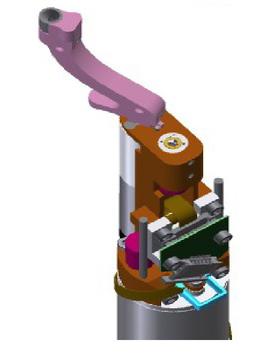
\includegraphics[scale=0.3]{images/realPositioner.jpg}
			\caption{CAD positioner model}
			\label{MOONS_positioner_representation}
		\end{minipage}
		\begin{minipage}[t]{5cm}
			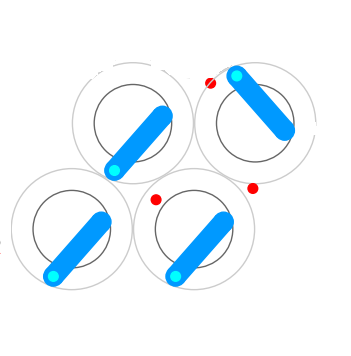
\includegraphics[scale=0.56]{images/MOONSPositioner_Simulation.png}
			\caption{MOONS positioner in simulation}
			\label{MOONS_positioner_simulation}
		\end{minipage}
		\begin{minipage}[t]{5cm}
			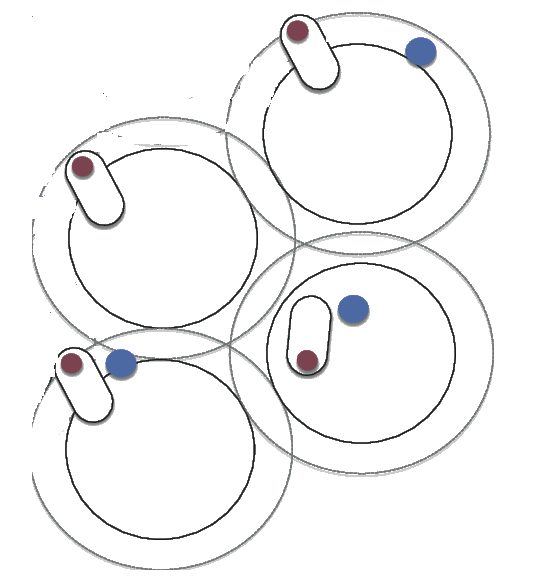
\includegraphics[scale=0.3]{images/DESI_Positioner.png}
			\caption{DESI positioner in simulation}
			\label{DESI_positioner_representation}
		\end{minipage}
	\end{figure}
			
	Though desirable, having a non complete system is not a serious issue since not all astronomical objects contain the same valuable information to study the universe evolution. Astronomers prefer to prioritize the observation of the important targets even at the price of disregarding the less relevant ones.
	
	With MOONS framework and as an extension of the previous work using a decentralized navigation function for collision avoidance [\citenum{MakaremMoons}], this paper explores an approach, through a finite state machine strategy, to take into account the importance/priority of each positioner's target into the coordination of their movements. As it gives more chance for higher priority positioners to reach their targets, its other objective is also to increase the positioners convergence with the goal of having a complete system.\\
		
	The organization of this paper is as followed: In section \ref{PRIORITY BASED COORDINATION}, a representation of the system and the finite state machine is described. Then we explain how deadlocks are localized and solved using an heuristic vector-distance based strategy. Section \ref{RESULTS} then presents the result of our approach on various test cases of positioner-configuration. As a conclusion, future research and possible improvements are discussed in section \ref{CONCLUSION}.
	
	\section{PRIORITY BASED COORDINATION}
	\label{PRIORITY BASED COORDINATION}
	
	
	Unlike many motion planning algorithms, the choice of using potential field to move simultaneously thousand of positioners stems from its time complexity and simplicity. It enables fast pre-computation of their anti-collision movements towards their targets. However, due to local minimum problems, using simple potential field to handle more complex systems which can exhibit deadlock situations prove to be complicated: it requires either a more complex development of the algorithm or an additional layer of complexity.\\\\
	In this work, we design a decision layer using a finite state machine which is built on top of a decentralized navigation function algorithm. It's role is to manage the interaction of positioners with their neighbour positioners having different orders of priorities. 

	\subsection{System representation}	
		\label{Finite-state machine} 
	
	Before explaining our approach, we need to establish how the system with priorities is defined. 
	 A depiction of the MOONS positioner and its equivalent in simulation are shown in figure \ref{MOONS_positioner_representation} - \ref{MOONS_positioner_simulation} - \ref{sys_representation}, where only the second arm (corresponding to the curve segment of the CAD model) is represented. The red dot is the target pre-assigned to the positioner's end-effector which holds the optic fiber represented by the dot at the extremity of the second arm.
		\begin{figure}[H]
			\centering
			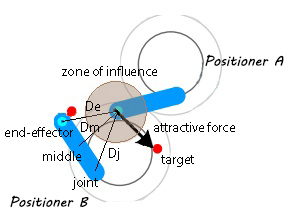
\includegraphics[scale=0.56]{images/system_representation.jpg}
			\caption{Variables representation of the system}
			\label{sys_representation}
		\end{figure}
	
	Let $p =$ \{$1,2,3,4$\} be the pre-assigned priority of a positioner, with 4 for the most important target and 1 the less important one. \\
	$D=$\{$D_e, D_m, D_j$\} is the set of distance between respectively the end-effector, middle and joint part of one positioner to another one's part. In figure \ref{sys_representation}, these distances are represented from positioner B to only the end-effector part of positioner A.\\\\
	As dictated by the principle of the potential field, each positioner is drawn to its target by an attractive force $F_a$ and avoiding its $i^{ieme}$ neighouring positioners with a repulsive forces, $F_{ri}$. Further details on their implementations in the context of MOONS are given in [\citenum{MakaremMoons}]. \\
	 With more than thousand positioners in a compact space and with each one having at most 6 neighbours, a "zone of influence", $Z_{F_{r}}$, is used for the repulsive forces. They are active only within this zone to limit and simplify the number of forces felt by one positioner from the others.\\ 
	 The zone $Z_{F_{r}}$ can be of any shape, but in this work, it was decided to be a circle around each part (end-effector, middle and joint) in order to have a simple cover on the whole positioner. The source of the repulsive force comes from the part of the neighbour positioner that is inside the zone $Z_{F_{r}}$.\\
	 
	\subsection{Finite-state machine}	
	
	The finite state machine has a total of 5 states with their corresponding transitions. Designed to take into account different priority values, it regulates the positioners interactions for a better coordination of the system.
	\subsubsection{First State: ON/OFF}
	\label{first_state_chap}
	The first state  is defined as the "ON/OFF" state. With the creation of a "ON/OFF zone", $Z_{ON/OFF}$, associated to a positioner, any neighbour positioners with a lower priority inside will have their attractive forces towards their targets disabled, ie $F_a = 0$. We refer to such a positioner as an OFF one in opposition to an ON one with its attractive force still active.
	Similarly to the influence zone $Z_{F_{r}}$, we use the same circle shape for $Z_{ON/OFF}$, centered on all the parts of the positioner in order to entirely cover it.\\\\
	 With only repulsive forces to prevent collision, it allows the ON positioner with the biggest priority to circulate through its OFF neighbours with less resistance, being the only one with an attractive force. This principle using priorities to solve the potential field local minima is illustrated in figure \ref{First_state}. 	
	\begin{figure}[H]
		\centering
		\begin{minipage}[t]{6.5cm}
			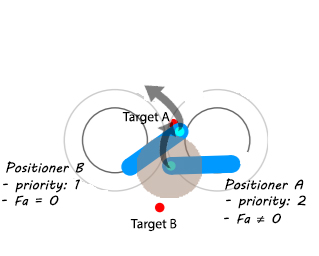
\includegraphics[scale=0.54]{images/first_state_0.jpg}
		\end{minipage}
		\begin{minipage}[t]{5cm}
			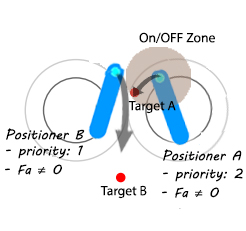
\includegraphics[scale=0.54]{images/first_state_ONOFF2.jpg}
		\end{minipage}
		\caption{\centering Principle of ON/OFF state (left to right image): \\
			(left image) Positioner B inside  $Z_{ON/OFF}$ of positioner A doesn't have any attrative force and is subject to repulsive force from positioner A, making it going to the opposite direction of its target B; (right image) The same positioner B, once repulsed outside of the zone $Z_{ON/OFF}$  by positioner A itself, regains its attractive force\\
\label{key}			}
		\label{First_state}
	\end{figure}
	
	A direct consequence of using only this state is the problem of deadlock due to oscillations at the limit of the zone $Z_{ON/OFF}$. Considering an ON positioner A and its OFF neighbour B with lower priority inside the zone $Z_{ON/OFF}$ of A (figure \ref{First_state} right image), when the positioner B is at the border of the zone, it can be subject to the problem of reactivation and deactivation of its attractive force. If the reactivated attractive force is opposing the movement of the positioner A, it will re-enter the zone $Z_{ON/OFF}$ of A only to be repulsed again. This switching state process can block the positioner A as the neighbour positioner B will keep oscillating at the same place.\\
	
	A deadlock can be interpreted as at least two positioners that stop moving towards their targets because of each other oscillating indefinitely at the same place in space. A moving average filter on the positioner's velocity can be used to  localize and unblock this situation by adding noise from it. Though it might be tempting to modify the magnitude of the different forces or of the noise, one has to consider the risk of collisions due to positioners sudden increase of velocity. \\
	Furthermore, only evaluating the velocity is necessary but not sufficient to detect a deadlock as explain later in the sub-chapter \ref{sub_chapter_fifth_state} since positioners can have a null velocity when arrived or when repulsing another one. \\\\
	With $v[t]$ the velocity of one positioner at time $t$, $y[t]$ is the output of the average moving filter of window $M$ such as:
	\begin{equation}
	\left\{
	\begin{IEEEeqnarraybox}[
	\IEEEeqnarraystrutmode
	\IEEEeqnarraystrutsizeadd{2pt}
	{2pt}
	][c]{rCl}
	y[t]& = & \dfrac{1}{M}\sum_{k=1}^{M}v[t-k]\\
	y[t] & < & thres \Rightarrow noise
	\end{IEEEeqnarraybox}
	\, \right.
	\label{}
	\end{equation} 
	We define $thres$, which value is defined experimentally, as the threshold representing when the positioner can be considered as "stopped".
	The result $y[t]$ is used to introduce noise once it is under this threshold. 
		
	\subsubsection{Second \& third state: ID and Priority memorization}
	Having introduced new variables with the first state, we need to determine how positioners interact with each others depending not only on their pre-assigned priority but also on their  ON and OFF states.\\\\
	As for the reason, problematic situations can also occur with the interaction of more than two positioners. Similarly to the positioner configuration illustrated in figure \ref{ID_PR} (left image), deadlock can happen when two ON high priority positioners A and B are going against each other by propagating their oppposite movements through an intermediate low priority OFF positioner C that is in-between them.\\
	
	In order to solve this problem and also for a better coordination of the system, we use the principle of memorization by introducing two new states: 
	\begin{itemize}
		\item "MemPr":  \\
		Initialized at 0 for a positioner, it is used to memorize either the pre-assigned priority or the MemPr of its neighbour positioner which changed its  states.\\
		\item "MemId": \\
		Initialized at 0 for a positioner, it is used to memorize only the identity of its neighbour positioner which changed its states.
	\end{itemize}\\
	  With this information and in a similar situation than in figure \ref{ID_PR}, one OFF positioner C, whose states has been changed by an ON neighbour positioner A due to its higher priority, is now able to influence its other ON neighbours states if their pre-assigned priorities are smaller than "MemPr" of C. The positioner A which changed the state of positioner C has its pre-assigned priority memorized by C. It enables the positioner A, through C, to influence other positioners whose movements are opposing its one, allowing to have its convergence to its target with less resistance.\\
	 We define this process as a "chain reaction": one OFF positioner being able to change the states of its neighbour positioner that is not the one that originally influenced it. \\
	 
	 To understand this principle and the assignments of values for "MemPr"  and "MemId", the pseudo-code of algorithm \ref{First_algo} gives a concise overview on how all the states seen so far for an considered positioner, called agent positioner, are changed when interacting with one of its neighbour. A visual step-by-step example following the algorithm \ref{First_algo} is illustrated in figure \ref{ID_PR}. \\\\
	 Furthermore, these rules are only valid if the agent positioner has not yet arrived to its target and is inside the $Z_{ON/OFF}$ zone of its considered neighbour.  
	 A condition related to another positioner state, the fourth one, that will be fully understand, as well as the whole condition in line \ref{arr_condition_line}, in the next sub-chapter \ref{sub_chap_fourth_state}.\\\\
 	\begin{figure}[H]
 		\centering
 		\begin{minipage}[t]{5.2cm}

 			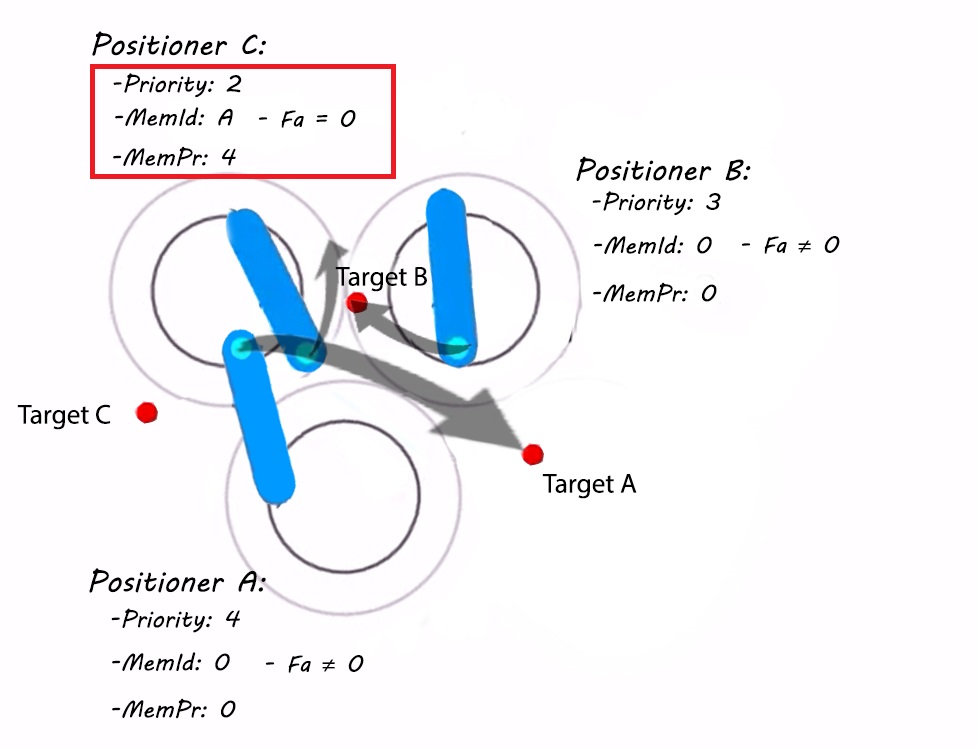
\includegraphics[scale=0.3]{images/ID_PR0.jpg}
 			\label{ID_PR0}
 		\end{minipage}
 		\begin{minipage}[t]{5.4cm}
 			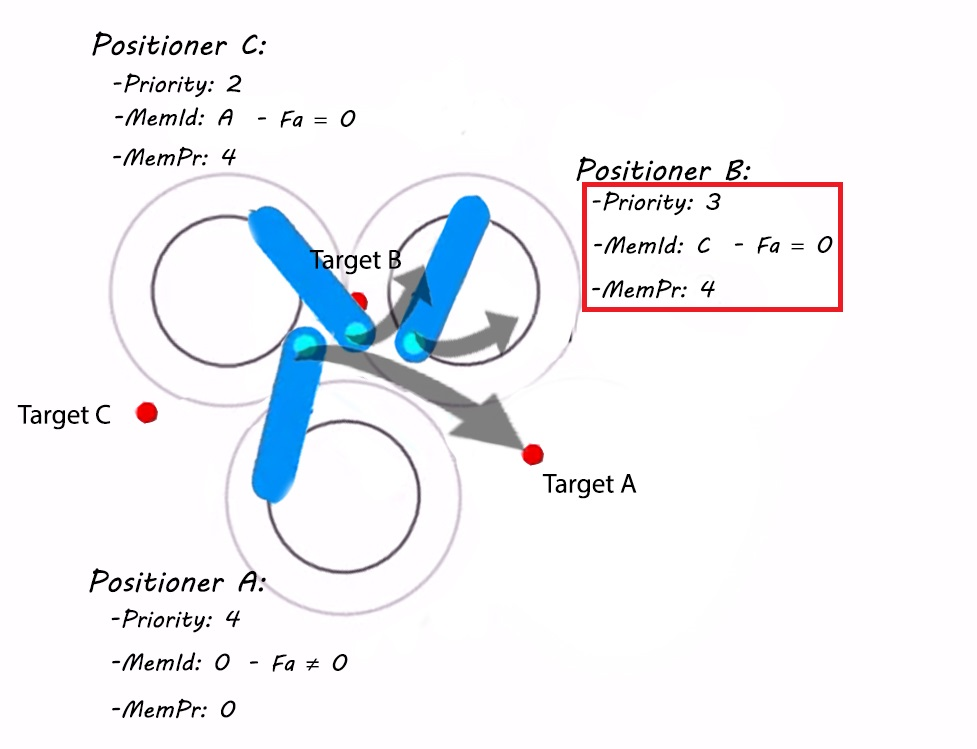
\includegraphics[scale=0.3]{images/ID_PR1.jpg}
 			\label{ID_PR1}
 		\end{minipage}
 		\begin{minipage}[t]{5.4cm}
 			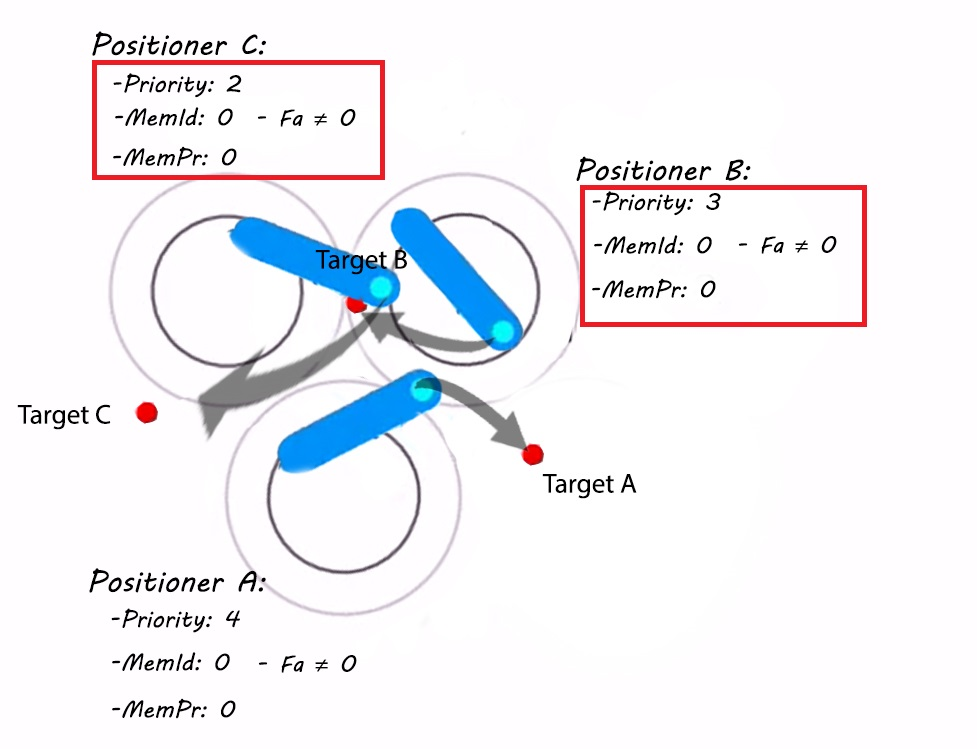
\includegraphics[scale=0.3]{images/ID_PR2.jpg}
 			\label{ID_PR2}
 		\end{minipage}
 		\caption{\centering Positioner chain reaction using MemId and MemPr states, obeying algorithm \ref{First_algo} for interaction:\\
 			(left image) Positioner A with the biggest priority influences its neighbour positioner C which remembers the priority and id information of A when becoming OFF; (middle image) Even if positioner C pre-assigned priority is smaller than B one, because C is OFF, B has to look on the memorized information of C: B having a smaller pre-assigned priority, it becomes OFF and carry on the memorized priority of C; (right image) Once positioner A is out of the zone $Z_{ON/OFF}$ of C, deep first search is used to reset all the states of all the positioners that are in the chain reaction because of A }
 		\label{ID_PR}
 	\end{figure}
	   The four main conditions in lines \ref{condition1}, \ref{condition2}, \ref{condition3}, \ref{condition4}, in the algorithm \ref{First_algo} correspond to all the possible interactions of two positioners based on their ON/OFF states. It shows how the neighbour positioner states is compared and is changing the agent positioner ones. Only the agent positioner states are modified. The reason is simply because algorithm \ref{First_algo} is applied to each positioner with respect to each of its neighours in the system.\\
	 
	The general rule of comparison for the priorities in line \ref{comparison1}, \ref{comparison2}, \ref{comparison3}, \ref{comparison4} depends on the ON/OFF state of the positioner: if the positioner is ON, the pre-assigned priority is used, otherwise it is the memorized priority "MemPr". Similarly, the possible values that can be assigned for the state "MemPr" of the agent positioner as shown in the lines after those conditions also depend on the first state ON/OFF of the neighbour positioner: the pre-assigned priority of the neighbour positioner if ON, else its "MemPr" priority.\\
	Therefore, all OFF positioners in the chain reaction remember the pre-assigned priority of the only ON positioner which is at the origin of this chain.\\\\	
	In all cases, the agent positioner always remember the ID of the neighbour positioner. It is used to track down all the positioners responsible for the chain reaction.   
	\begin{algorithm}[H]
		\caption{agent\_status($agent$, $neighbour$)}\label{AlgoRedSoftEnve}
		\label{First_algo}
		\SetKwData{Left}{left}\SetKwData{This}{this}\SetKwData{Up}{up}
		\SetKwFunction{Union}{Union}\SetKwFunction{FindCompress}{FindCompress}
		\SetKwInOut{Input}{input}\SetKwInOut{Output}{output}
		\Output{For a considered positioner, called agent positioners, modification of its 1st, 2nd and 3rd states with respect to its considered neighbour positioner }
		
		\BlankLine
		\setcounter{AlgoLine}{0}
		\SetAlgoLined
		\uIf{agent.Arr == False  or neighbour == OFF \tcp*{"Arr" state introduced on sub-chapter \ref{sub_chap_fourth_state}}   \label{arr_condition_line} } 
		{		\BlankLine
			\uIf{agent == OFF and neighbour == OFF \label{condition1}}{
						\BlankLine
				\uIf{agent.MemPr $<$ neighbour.MemPr \label{comparison1}}{
					\BlankLine
					agent.MemId =  Neighbour Id\;\\
					agent.MemPr =  Neighbour.MemPr\;\\
				}
			}
			\uElseIf{agent == ON and neighbour == ON \label{condition2}}{
						\BlankLine
				\uIf{Agent Priority $<$ Neighbour Priority \label{comparison2}}{
					\BlankLine
					agent.ON/OFF = OFF \;\\
					agent.MemId =  Neighbour Id\;\\
					agent.MemPr =  Neighbour Priority\;\\
				}
			}
			\uElseIf{agent == OFF and neighbour == ON \label{condition3}}{
						\BlankLine
				\uIf{agent.MemPr $<$ Neighbour Priority \label{comparison3}}{
					\BlankLine
					agent.MemId =  Neighbour Id\;\\
					agent.MemPr =  Neighbour Priority\;\\
				}
			}
			\uElseIf{agent == ON and neighbour == OFF \label{condition4}}{
						\BlankLine
				\uIf{Agent Priority $<$ neighbour.MemPr \label{comparison4}}{
					\BlankLine
					 agent.ON/OFF = OFF \;\\
					agent.MemId =  Neighbour Id\;\\
					agent.MemPr =  Neighbour.MemPr\;
				}
			}
						\BlankLine
			\uIf{agent.MemId == Neighbour ID\label{conditionSame}}{
				\BlankLine
				Return indication Agent positioner states still being changed !
			}
	}
		\BlankLine
	\end{algorithm}
	
	 The lifetime of the memorization states, "MemId" and "MemPr", is bound to its agent positioner being OFF inside the $Z_{ON/OFF}$ zone of the neighbour positioner that changed its states. Once outside, its states are re-initialized at their initial values, i.e. the first state at ON and the memorization states at 0. The states of all the other positioners that were influenced by the re-initiliazed agent positioner through the chain reaction process are also re-initialized. To do so, deep first search algorithm can be used with the "MemId" information to recognize which positioner is in the chain reaction.\\\\
	When the algorithm \ref{First_algo} is reapplied again on the same two positioners, the agent positioner inside the $Z_{ON/OFF}$ zone of its neighbour positioner won't enter any of the conditions mentionned above since its states were already changed previously by this same neighbour. The condition in line \ref{conditionSame} is added to ouptut that the agent positioner is still being affected by the same neighbour positioner, in order to avoid any complicated behaviors of the system.  

	
	\subsubsection{Fourth state: Arrived}
	\label{sub_chap_fourth_state}
	With the supposition that a positioner with the highest priority, $p = 4$, is already at destination, any lower priority positioners with their targets inside its zones $Z_{ON/OFF}$ and $Z_{F_{r}}$  are subject to repulsion forces and a changes of their states. The results are their attractive forces being disabled once inside the zones and the positioners being repulsed without resistance, hence never reaching their targets.\\
	\\
	This particular oscillation scenario is shown in figure \ref{fourth_state} with a the positioner A having a higher pre-assigned priority than a positioner B whose target is inside the zones of A. Once inside the $Z_{ON/OFF}$ and $Z_{F_{r}}$, the positioner B, changing to OFF, will have its attractive force deactivate and repulsed.
	\begin{figure}[H]
		\centering
		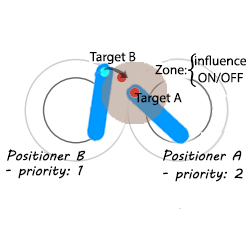
\includegraphics[scale=0.64]{images/fourth_state.jpg}
		\caption{\centering	Principle of fourth state "Arr":\\
		Problematic configuration with target inside a higher priority "already-converged" positione zones $Z_{ON/OFF}$ and $Z_{F_{r}}$ }
		\label{fourth_state}
	\end{figure}
	In order to solve this problematic behavior, a fourth state, "Arr", is introduced to qualify a positioner that has converged to its target. \\\\
	Coming with this new state is the inability for the already converged positioner A to affect any other positioners states which are inside its zone $Z_{ON/OFF}$, regardless of their priorities.
	Without having their attractive forces canceled, the neighbour positioners can converge to their targets that are inside the zone.\\\\
	In addition, the zone $Z_{F_{r}}$ has to be mitigated such that the repulsive forces felt from the neighbour positioners do not hinder their convergences. Although several complex methods can be used, we decided to simply reduce the radius of the repulsion zone $Z_{F_{r}}$. Though two very close targets can make two positioners oscillates a little bit as the one arriving might repulse the one already arrived, both can stabilize and converge surprisingly well by adding some dead-zone between the end-effector and its target or time delay before the positioner exit its "Arr" state.  
	
	\subsubsection{Fifth state: Deadlock and pseudo-priority}
	\label{sub_chapter_fifth_state}
	In order to have a clearer and better explanation of this fifth state, this sub-chapter will be divided in three part: 
	\begin{enumerate}
		\item A description of its state and principle by first illustrating it with an example on with the real world traffic circulation. The objective of this analogy is to enable a better understanding on how this state was designed.
		\item An explanation on how the state changes when interacting with other positioners
		\item Finally how to detect situations which require its activation
	\end{enumerate}
	
	\paragraph{State and Principle}\mbox{}\\
	
	So far, the finite state machine only takes into account direct positioner interaction with different priorities.
	When two positioners with same priority and opposite movement direction enter in direct contact, deadlock situation is more highly to occur. This scenario is the reason why a fifth and last state is added to the finite state machine, to regulate the direct interaction between positioners with same priority.\\\\	
	To better understand the design of this state introduced below and also to have a better understanding of it principles, we can take as an example the well known problem of trafic jam where two vehicles are being blocked by each other at one intersection. Of course, an ambulance in this scenario would have had the priority over the other vehicles, which is why we assume that they are two same vehicle equally important.\\
	Usually in this kind of situation, the first goal of the drivers is not anymore to reach their targets but instead to find a solution to the actual problem, while monitoring if any important vehicle such as an ambulance or a military tank is approching (so they can quickly go off-route into the sidewalk for example to let them pass).\\ 
	To solve this problem, they just "isolate" themselves from the rest (as involving more vehicles will only make the situation more complicated to solve) to better find a solution by dertermining which one should have the priority over the other. 
	To do so, each one is assessing the situation based on their own perspective and the code road rules to determine which one should go first, usually depending on which direction they wanted to go at the beginning.\\
	
	
	With this example in mind, we define "lock\_sm" as the fifth state to designate if its positioner is in a deadlock situation with another one that has the same priority. For the rest of this paper, we refer to this specific situation as a "lock\_sm" situation. \\\\
	In addition, a pseudo-priority variable, "psPr", is also associated to each positioner to enable the system to obey the following principle, as illustrated in figure \ref{5thState}:\\
	When in a "lock\_sm" situation, the first priority of the two positioners is not to reach their targets anymore but instead to solve their current problem by determining which one should have the priority over the other. To do so, both their distances from their end-effector to their respective targets are evaluated such that, in orded to solve this situation more quickly, the positioner with the smallest distance becomes more important. The idea is to have the pseudo-priority, "psPr", for only the  "lock\_sm" situation, in order to indicate which of the two positioners is more important while the interactions with the other positioners is regulated with the pre-assigned priority. \\\\
	Moreover, to facilitate the movement into solving the deadlock problem, the positioner with bigger pseudo-priority is having an additional isotropic and constant repulsive force from the target of the other positioner that is in a "lock\_sm" situation with it, which can be formulated as a direct weighted relation with the current velocity of the positioner.\\\\
	
	\begin{figure}[H]
		\centering
		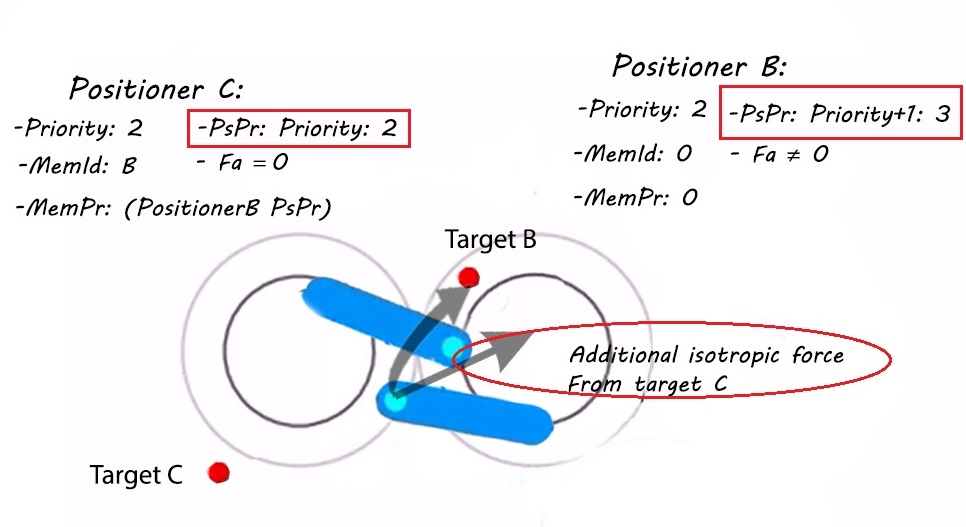
\includegraphics[scale=0.4]{images/5thstate.jpg}
		\caption{\centering Principle of 5th state, "lock\_sm", and pseudo-priority, "psPr" :\\
		With the same priority, inside their zone "$Z_{ON/OFF}$" and in "lock\_sm" situation, the distance from positioner B end-effector to its target being smaller compared to the end-effector C to target C, the positioner B becomes more important symbolised by its pseudo-priority, "PsPr", being bigger and both fifth state equal to B}
		\label{5thState}
	\end{figure}
		
	Initialize at 0 and at the pre-assigned priority of the positioner for respectively the "lock\_sm" state and the pseudo-priority, "psPr",  these states change when being inside the zone "$Z_{ON/OFF}$" and the configuration of the two positioners is considered leading to a deadlock situation. \\
	In case of a "lock\_sm" situation, the pseudo-priority of the positioner deemed the most important one is increase by 1, while both positioner's fifth state "lock\_sm" is equal to the ID of the most important positioner. The reason is to give an unique identification to each  "lock\_sm" problem between two positioners.
	
	

%	\paragraph{Positioner interaction}\mbox{}\\
%	Having define the new state principle, the question of how the interactions is done with the positioners and when to consider a situation to be a "lock\_sm" deadlock is answered in the following paragraph.	
	\paragraph{Deadlock localization}\mbox{}\\
	In order to localize a deadlock, we use the point of view from both the closest parts (end-effector, middle or joint) of the two positioners with equal pre-assigned priority inside the zone " $Z_{ON/OFF}$". The objectif is to evaluate if they could possibly create a  "lock\_sm"  situation.\\
	Considering an agent and neighbour positioner with equal priority, the point of view can be understood as how the agent is seeing its target and its neighbours target with respect to its neighbours positioners closest part. 
	Mathematically, we define it as the projection of the agent and neighbour target on the line created by the vector between the closest parts of both positioners that could possibly be responsible for the deadlock situation.\\
	
	\begin{figure}[H]
		\centering
		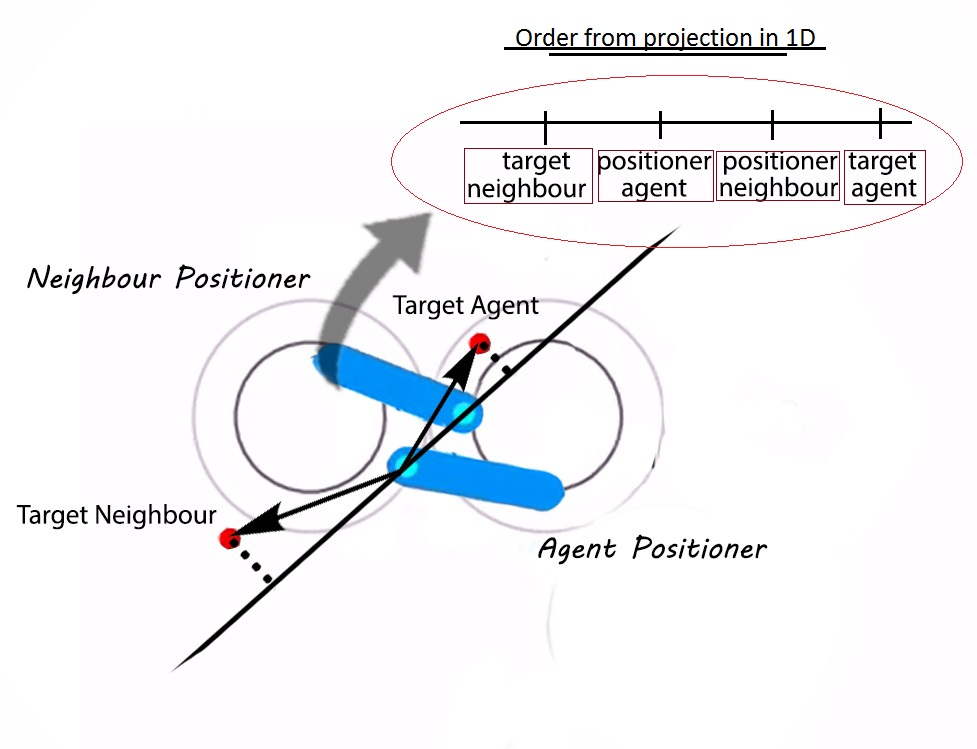
\includegraphics[scale=0.4]{images/Projection1.jpg}
		\caption{\centering 1D configuration:\\
			 Projection of agent and neighbour target on line created from closest part of both positioners}
		\label{projection}
	\end{figure}
	
	It basically projects everything into a line in order to evaluate in 1D if the agent target is on the same side as the agent positioner or is behind the neighbour positioner. For the latter case as shown in figure \ref{projection}, the neighbour positioner then becomes an obstacle to the movement of the agent one, possible leading to a deadlock situation.
	Since the movement of the positioner is planar with 2 degree of freedom, having the point of view from both positioners allows a better perspective of the current configuration.\\\\
	In order to assess if the 1D configuration obtained from projection is considered a deadlock situation, we compare the resulting 1D projection result with a look-up table that corresponds to all possible 1D configurations of the agent, neighbour positioners and their targets placed in 1 line, so all 24 possible permutations.
	The logic behind to distinguish which configuration is considered a deadlock is simply to individually assess for each configuration if they are any collision in both positioners movements towards their target on the 1D line. The example as seen in figure \ref{look_UpTableLogic} shows few reasoning examples that can be generalize to determine the rest of the 1D configurations.
	\begin{figure}[H]
		\centering
		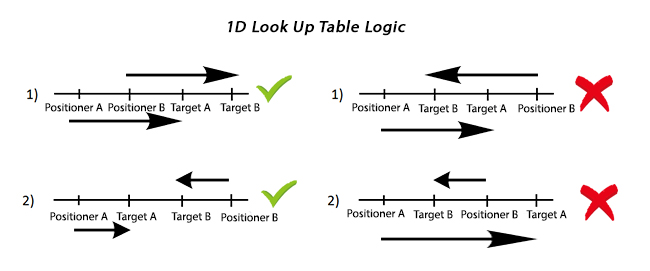
\includegraphics[scale=0.55]{images/1DLookUpTable.jpg}
		\caption{\centering
			 Configuration examples of look up table logic:\\
			On the left column, positioner A and B movements are not opposing each other nor are the positioner on the way of the other movement; 
			On the right column,  the positioner B ending up at its target will hinder the movement of positioner A to its target, being in between them }
		\label{look_UpTableLogic}
	\end{figure}
	\section{Simulation \& RESULTS}
	\label{RESULTS}
	\subsection{Software \& Hardware}
	\label{Software Hardware}
	To evaluate our approach, a simulator developed in python which recreates the shape and the behavior of the positioners is used. The trajectories of the positioners are first pre-computed and then directly given in open-loop to the electronics controlling the motors.\\  
	All simulation tests were conducted on a Lenovo thinkpad T450s with an Intel Core i7-5600U @ 2.69GHz x 4 processor, GeForce 940M SSE2 graphic card on an ubuntu 14.04 LTS version.
	\subsection{Tests \& results}
	\label{Test cases}
	
	Repeatability tests are done in order to assess the performance and efficiency of our approach. For this purpose, we compare the results obtained from our finite state machine (FSM) with the ones using only the decentralized navigation function algorithm (Without FSM). In the latter case, pre-assigned priorities are not taken into account as they are no mechanism to do so.\\\\
	In addition to all the figures seen so far which are real working examples of different priorities positioner interaction, the goal is also to assess the robustness of the algorithm to coordinate a whole system of positioners with a hierarchy of importance.
	
	\subsubsection{Repeatability: convergence and time performance}
	We run our algorithm on 8 different test files. Each represents one specific and unique initial configuration of thousand of positioners with their respective targets. All positioners have the same pre-assigned priority value.\\\\
	Each configuration file is used to evaluate the following performances: 
	\begin{itemize}
		\item Number of positioners successfully converging to their targets.
		\item Time in seconds necessary for the pre-computation of their movements.
	\end{itemize}
	The goal is not only to verify if the performance of our algorithm is repeatable over different configurations of our system but also if it is acceptable to use it in real time.\\
	To this end, for each configuration test file, the total number of around a thousand of positioners is partitioned into 12 subsets of sub-total positioners, on which we run our algorithm. The results are given in figures \ref{configuration1_result}, \ref{configuration2_result}, \ref{configuration3_result}, \ref{configuration4_result}, \ref{configuration5_result}, \ref{configuration6_result}, \ref{configuration7_result}, \ref{configuration8_result}.
	
	\begin{figure}[H]
		\begin{minipage}{8.7cm}
			\begin{minipage}[t]{4.3cm}
				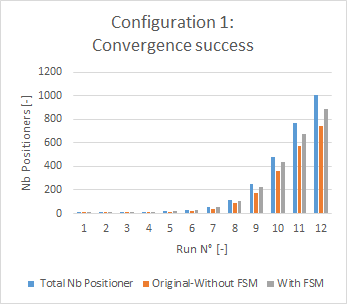
\includegraphics[scale=0.56]{images/configuration1_conv}
				\label{configuration1_conv}
			\end{minipage}
			\begin{minipage}[t]{1.0cm}
				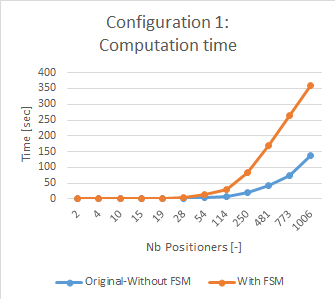
\includegraphics[scale=0.57]{images/configuration1_time}
				\label{configuration1_time}
			\end{minipage}
			\caption{\centering Configuration 1:\\
				 Convergence success and computation time data
				 \begin{itemize}
	 					 	\item With FSM: Decentralized navigation function with finite state machine
	 					 	\item Without FSM: Decentralized navigation function without finite state machine
				 \end{itemize}
			\tiny
			\begin{tabular}{|l|l|l|l|l|l|l|l|}
					\hline
					\multicolumn{2}{|l|}{Total Positioners}  & 54 & 114 & 250 & 481 & 773 & 1006\\
					\hline
					Conv. & With FSM  & 52 & 105  & 228 & 434 & 675 & 889 \\
					\cline{2-8}
						 & Without FSM & 41  & 88 & 176 & 358 & 577 & 747 \\
					\hline
					Time\\(sec) & With FSM  & 13.8 & 30.9  & 84 & 169.7 & 265.2 & 360.1 \\
					\cline{2-8}
					& Without FSM  & 3.5  & 8.6 & 21.4 & 43.7 & 74.5  & 136.1 \\
					\hline
			\end{tabular}}
				\label{configuration1_result}
		\end{minipage}
		\begin{minipage}{9cm}
			\begin{minipage}[t]{4.2cm}
				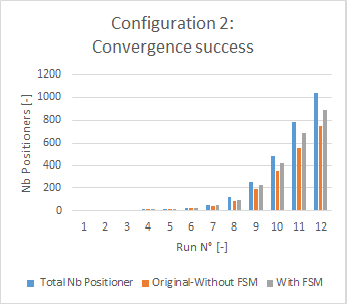
\includegraphics[scale=0.56]{images/configuration2_conv}
				\label{configuration1_conv}
			\end{minipage}
			\begin{minipage}[t]{1.0cm}
				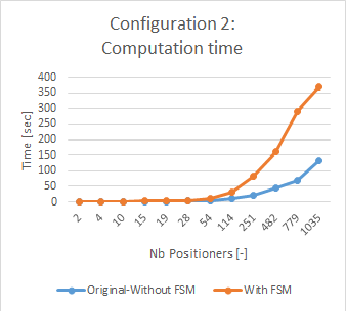
\includegraphics[scale=0.56]{images/configuration2_time}
				\label{configuration1_time}
			\end{minipage}
			\caption{\centering Configuration 2:\\
				Convergence success and computation time data
				 \begin{itemize}
							 	\item With FSM: Decentralized navigation function with finite state machine
							 	\item Without FSM: Decentralized navigation function without finite state machine
				 \end{itemize}
							\tiny
				\begin{tabular}{|l|l|l|l|l|l|l|l|}
					\hline
					\multicolumn{2}{|l|}{Total Positioners}  & 54 & 114 & 251 & 482 & 779 & 1035\\
					\hline
					Conv. & With FSM  & 52 & 103  & 231 & 415 & 679 & 892 \\
					\cline{2-8}
					& Without FSM & 45  & 91 & 189 & 350 & 555 & 750 \\
					\hline
					Time\\(sec) & With FSM  & 11.8 & 31  & 81.2 & 159.2 & 291.7 & 369.7 \\
					\cline{2-8}
					& Without FSM  & 3.8  & 9.6 & 21.6 & 44 & 69.9  & 134.1 \\
					\hline
				\end{tabular}
				}
			\label{configuration2_result}
			\end{minipage}
	\end{figure}
\begin{figure}[H]
	\begin{minipage}{8.7cm}
		\begin{minipage}[t]{4.3cm}
			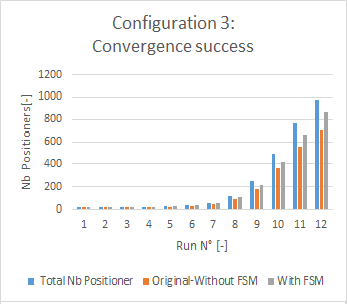
\includegraphics[scale=0.56]{images/configuration3_conv}
			\label{configuration1_conv}
		\end{minipage}
		\begin{minipage}[t]{1.0cm}
			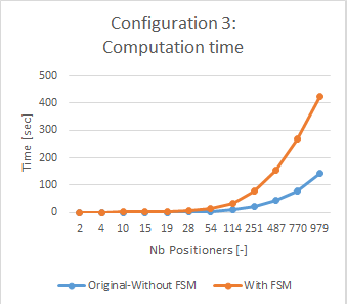
\includegraphics[scale=0.57]{images/configuration3_time}
			\label{configuration1_time}
		\end{minipage}
		\caption{\centering Configuration 3:\\
			Convergence success and computation time data
			\tiny
			\begin{tabular}{|l|l|l|l|l|l|l|l|}
				\hline
				\multicolumn{2}{|l|}{Total Positioners}  & 54 & 114 & 251 & 487 & 770 & 979\\
				\hline
				Conv. & With FSM  & 53 & 101  & 217 & 413 & 665 & 864 \\
				\cline{2-8}
				& Without FSM & 41  & 86 & 181 & 358 & 554 & 704 \\
				\hline
				Time\\(sec) & With FSM  & 14 & 32.3  & 79.9 & 155.1 & 267.2 & 425.2 \\
				\cline{2-8}
				& Without FSM  & 3.7  & 9.1 & 21 & 45.2 & 79.2  & 143.6 \\
				\hline
			\end{tabular}
			}
			\label{configuration3_result} 
		\end{minipage}
		\begin{minipage}{9cm}
			\begin{minipage}[t]{4.2cm}
				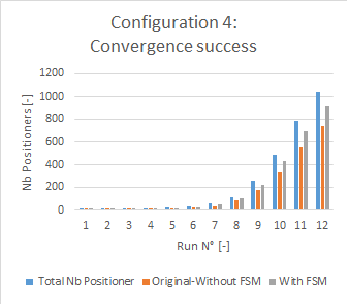
\includegraphics[scale=0.56]{images/configuration4_conv}
				\label{configuration1_conv}
			\end{minipage}
			\begin{minipage}[t]{1.0cm}
				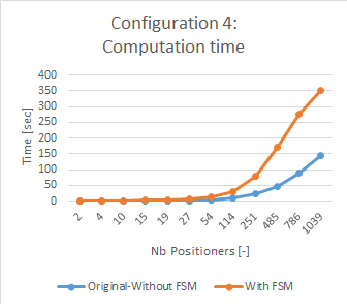
\includegraphics[scale=0.56]{images/configuration4_time}
				\label{configuration1_time}
			\end{minipage}
			\caption{\centering Configuration 4:\\
				Convergence success and computation time data
				\tiny
				\begin{tabular}{|l|l|l|l|l|l|l|l|}
					\hline
					\multicolumn{2}{|l|}{Total Positioners}  & 54 & 114 & 251 & 485 & 786 & 1039\\
					\hline
					Conv. & With FSM  & 48 & 103  & 222 & 436 & 698 & 914 \\
					\cline{2-8}
					& Without FSM & 35  & 81 & 172 & 339 & 553 & 742 \\
					\hline
					Time\\(sec) & With FSM  & 13.4 & 30.8 & 79.6 & 170.4 & 274.1 & 352.1 \\
					\cline{2-8}
					& Without FSM  & 3.8  & 9.3 & 23.9 & 47.3 & 89.5  & 144.9 \\
					\hline
				\end{tabular}
				}
				\label{configuration4_result} 
			\end{minipage}
		\end{figure}
\begin{figure}[H]
	\begin{minipage}{8.7cm}
		\begin{minipage}[t]{4.3cm}
			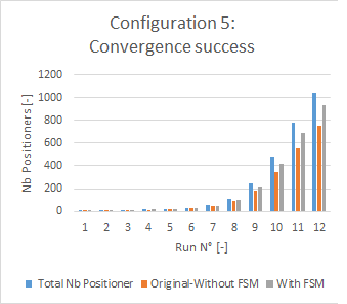
\includegraphics[scale=0.56]{images/configuration5_conv}
			\label{configuration1_conv}
		\end{minipage}
		\begin{minipage}[t]{1.0cm}
			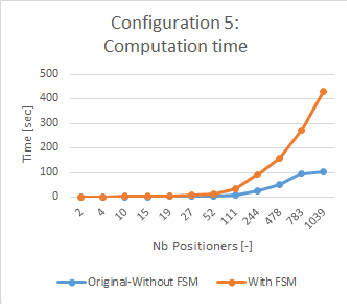
\includegraphics[scale=0.57]{images/configuration5_time}
			\label{configuration1_time}
		\end{minipage}
		\caption{\centering Configuration 5:\\
			Convergence success and computation time data
			\tiny
			\begin{tabular}{|l|l|l|l|l|l|l|l|}
				\hline
				\multicolumn{2}{|l|}{Total Positioners}  & 52 & 111 & 244 & 478 & 783 & 1039\\
				\hline
				Conv. & With FSM  & 50 & 105  & 219 & 421 & 689 & 931 \\
				\cline{2-8}
				& Without FSM & 44  & 89 & 186 & 349 & 555 & 754 \\
				\hline
				Time\\(sec) & With FSM  & 12.9 & 32.7  & 91.8 & 155.9 & 267.8 & 429.7 \\
				\cline{2-8}
				& Without FSM  & 3.8  & 8.7 & 24.1 & 47.2 & 93.3  & 103.4 \\
				\hline
			\end{tabular}
			}
			\label{configuration5_result} 
		\end{minipage}
		\begin{minipage}{9cm}
			\begin{minipage}[t]{4.2cm}
				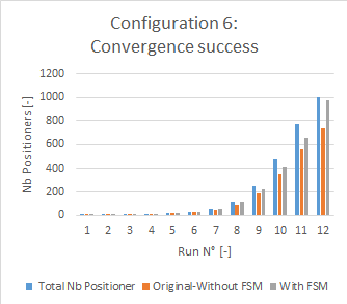
\includegraphics[scale=0.56]{images/configuration6_conv}
				\label{configuration1_conv}
			\end{minipage}
			\begin{minipage}[t]{1.0cm}
				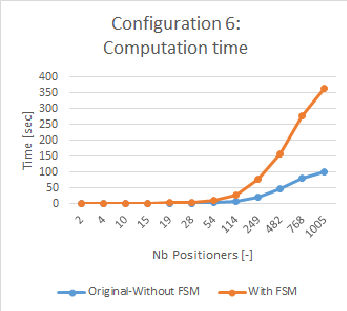
\includegraphics[scale=0.56]{images/configuration6_time}
				\label{configuration1_time}
			\end{minipage}
			\caption{\centering Configuration 6:\\
				Convergence success and computation time data
				\tiny
				\begin{tabular}{|l|l|l|l|l|l|l|l|}
					\hline
					\multicolumn{2}{|l|}{Total Positioners}  & 54 & 114 & 249 & 482 & 768 & 1005\\
					\hline
					Conv. & With FSM  & 54 & 110 & 225 & 415 & 651 & 973 \\
					\cline{2-8}
					& Without FSM & 47  & 90 & 187 & 356 & 561 & 734 \\
					\hline
					Time\\(sec) & With FSM  & 12 & 28.8 & 76.3 & 158.6 & 275.9 & 364.2 \\
					\cline{2-8}
					& Without FSM  & 3.9  & 8.6 & 22.6 & 46.4 & 79.8  & 101.2 \\
					\hline
				\end{tabular}
				}
				\label{configuration6_result} 
			\end{minipage}
		\end{figure}
\begin{figure}[H]
	\begin{minipage}{8.7cm}
		\begin{minipage}[t]{4.3cm}
			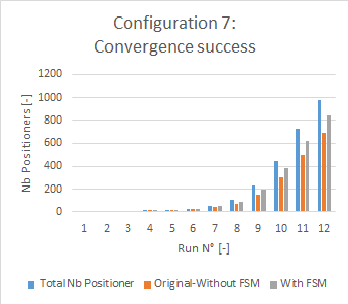
\includegraphics[scale=0.56]{images/configuration7_conv}
			\label{configuration1_conv}
		\end{minipage}
		\begin{minipage}[t]{1.0cm}
			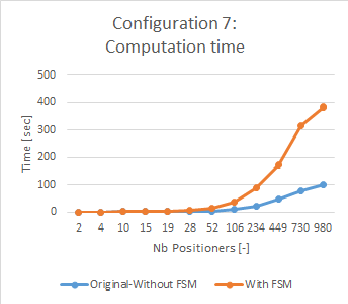
\includegraphics[scale=0.57]{images/configuration7_time}
			\label{configuration1_time}
		\end{minipage}
		\caption{\centering Configuration 7:\\
			Convergence success and computation time data
			\tiny
			\begin{tabular}{|l|l|l|l|l|l|l|l|}
				\hline
				\multicolumn{2}{|l|}{Total Positioners}  & 52 & 106 & 234 & 449 & 730 & 980\\
				\hline
				Conv. & With FSM  & 50 & 90  & 196 & 382 & 621 & 844 \\
				\cline{2-8}
				& Without FSM & 40  & 72 & 155 & 300 & 503 & 691 \\
				\hline
				Time\\(sec) & With FSM  & 14.4 & 36.2  & 89 & 172.8 & 315.8 & 383 \\
				\cline{2-8}
				& Without FSM  & 3.9  & 8.6 & 21.1 & 46.8 & 76.5  & 102.1 \\
				\hline
			\end{tabular}
			}
		\label{configuration7_result} 
		\end{minipage}
		\begin{minipage}{9cm}
			\begin{minipage}[t]{4.2cm}
				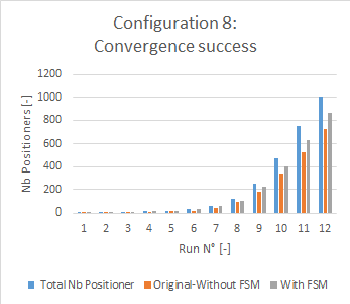
\includegraphics[scale=0.56]{images/configuration8_conv}
				\label{configuration1_conv}
			\end{minipage}
			\begin{minipage}[t]{1.0cm}
				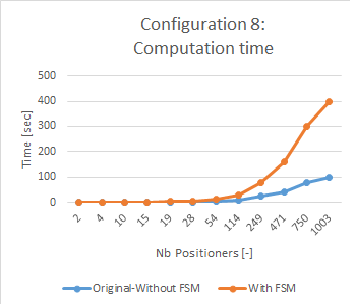
\includegraphics[scale=0.56]{images/configuration8_time}
				\label{configuration1_time}
			\end{minipage}
			\caption{\centering Configuration 8:\\
				Convergence success and computation time data
				\tiny
				\begin{tabular}{|l|l|l|l|l|l|l|l|}
					\hline
					\multicolumn{2}{|l|}{Total Positioners}  & 54 & 114 & 249 & 471 & 750 & 1003\\
					\hline
					Conv. & With FSM  & 52 & 103 & 221 & 401 & 630 & 861 \\
					\cline{2-8}
					& Without FSM & 40  & 86 & 179 & 342 & 525 & 723 \\
					\hline
					Time\\(sec) & With FSM  & 12.3 & 29.2 & 78.2 & 161.9 & 301.2 & 399.5 \\
					\cline{2-8}
					& Without FSM  & 4  & 9.2 & 23.0 & 42.7 & 78.3  & 99.5 \\
					\hline
				\end{tabular}}
				\label{configuration8_result} 
			\end{minipage}
		\end{figure}					
	For all the configuration tests, the general behavior of the system remains similar: when using our finite state machine, an improvement of positioners convergence from 60-70\% to 80-95\% can be observed globally and for each test.\\
	 However, the computation time is bigger, growing into a quasilinear order. It is an expected result since we added an another layer of computation to the already existing algorithm that we use for comparison. With better optimization such as parallel computation and/or more performant hardwares, this burden can be compensated.\\\\
	 Though all their pre-assigned priorities to each positioner are the same value, the result of convergence improvement with our method also demonstrates indirectly the robustness of our algorithm to take into account different priorities. Due to the mechanism of the fifth state of the finite machine, interactions of positioners with similar priorities also involves all the other states as their priorities become different. \\\\
%	\subsubsection{Special situations}
%	Test cases illustrated in [\citenum{TestCaseMoon}] and showcasing problematic positioners configurations, ie specifically designed situations where two or more positioners are supposed to fail reaching their targets with just using the decentralized navigation function due to deadlocks, are used to test our algorithm.\\
%	Unlike the test of repeatability, the goal here is to  
	
	
	\section{CONCLUSION}
	\label{CONCLUSION}
	In the context of the project MOONS and as an extension of [\citenum{MakaremMoons}], an approach with a finite state machine is built on top of a decentralized navigation function from the potential field family. It enables better coordination of a multi-objects positioners inside a confined space. With its different states, it takes into account different priorities pre-assigned to each positioner, creating a hierarchy of importance where positioners with higher priority have more probabilities to reach their targets. Along with the possibility to manage deadlocks, it enables a better convergence of the system:
	 an improvement from  60-70\% to 80-95\% of total positioners converging to their targets is observed from repeatability tests. The results are obtained from comparing our approach with the one using only the decentralized navigation function. Furthermore, the algorithm is scalable to other system configuration than MOONS as it doesn't depend on the positioner's geometry.\\
	Since we added another layer of complexity to an already existing algorithm, the pre-computation time of each positioner trajectory is slower, becoming quasilinear. One possible work can be to optimize the software by either finding the right optimization method such as parallel computing or using more performant hardwares. Moreover, since our approach has no proof of completeness, more research on the optimization of the algorithm for a better positioner convergence can be consider.\\
	Extending this approach to take into account other features, such as for the project SLOAN-SDSS5 that needs to select which (UV, visible or IR) optical fibers to use within one positioner is also a possibility. It is a subject which is particularly interesting for astronomers since not all objects in the universe are well observed in the same range of the optic spectrum.
	
	\acknowledgments % equivalent to \section*{ACKNOWLEDGMENTS}       
	
	I would like to thank my supervisor Dr. Denis Gillet for his patience and trust in me, and also to Dr. Mohammed Bouri and prof. Jean-Paul Kneib for their support. A lot of thanks to Ezequiel Gonzalez for our brainstorming sessions and to Dr. Laleh Makarem for reviewing my work and her advices, without whom this paper and algorithm wouldn't have been possible; and finally, to all the friendly members of the REACT Lab who made my working place a nice and productive environment. 
	

% References
\bibliography{report} % bibliography data in report.bib
\bibliographystyle{spiebib} % makes bibtex use spiebib.bst

\end{document} 
